\newpage





%
%
%  S  É  A  N  C  E     I
%
%



\section{Aide pour réaliser les activités}

\subsection{Aide pour la séance 1...}\label{correction_scratch1}




Nous allons écrire le programme étape par étape.


\subsubsection{Modifier la scène où se passe l'action}\index{Scratch!Modifier la scène}\index{Modifier la scène (Scratch)}

La scène correspond à l'arrière-plan (blanc au départ) où se passe l'action. La scène est un objet qui peut être modifié. Pour cela, la première étape est de cliquer sur l'icône scène 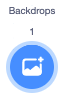
\includegraphics[width=1cm]{./images/scratch/changerScene} en bas à droite.

\uneimageici{./images/scratch/changerScene0.png}{.65\textwidth}

Une fois la scène sélectionnée (elle est alors entourée en couleur), suivre les 4 étapes suivantes :

\begin{enumerate}
\item Cliquer sur l'onglet \texttt{Choisir un arrière-plan}.
\item Chercher l'arrière-plan \texttt{Xy-grid}.
\item Cliquer sur l'arrière-plan \texttt{Xy-grid} pour remplacer le fond blanc qui était installé par défaut. 
\end{enumerate}

A noter qu'il est également possible d'\texttt{importer un arrière-plan} à partir d'images présentes sur votre ordinateur.

%\uneimageici{./images/scratch/ScratchChangerScene1}{.8\textwidth}

Notre programme comporte maintenant deux scènes différentes : \texttt{arrière-plan1} et \texttt{Xy-grid}. C'est cette dernière qui est sélectionnée (elle est entourée en couleur).

\uneimageici{./images/scratch/choixBackdrop.png}{.4\textwidth}






\subsubsection{Enregistrer le programme}\index{Enregistrer!Scratch}\index{Scratch!Enregistrer}

Pour enregistrer votre programme, cliquer sur \texttt{Sauvegarder sur votre ordinateur} :
%
\includegraphics[width=.4cm]{./images/scratch/Sauver} :

\uneimageici{./images/scratch/enregistrer_scratch.png}{.5\textwidth}

Le fichier s'enregistre alors par défaut au format .sb3 dans le dossier \texttt{Téléchargements} de votre ordinateur.\\

%Il faut ensuite choisir l'emplacement \emph{Bureau} de l'ordinateur, puis donner un nom au fichier dans lequel votre programme sera sauvegardé :

%\uneimageici{./images/scratch/ScratchEnregistrerProgramme2}{.7\textwidth}


Comme toujours en informatique, il ne faut pas oublier d'enregistrer régulièrement le travail. Pour cela, cliquer régulièrement sur \texttt{Sauvegarder sur votre ordinateur}.

%\uneimageici{./images/generales/clavierCmdS}{.4\textwidth}









\subsubsection{Ajouter un code associé au sprite}\label{ScriptLutin}\index{Scratch!Script associé à un objet}\index{Script associé à un objet (Scratch)}

Le sprite est un autre objet. C'est lui qui réalise l'action principale du programme. On va lui associer un programme (nommé \textbf{code}) qui contient une succession d'ordres (les \textbf{instructions}) qu'il devra réaliser.  \\

Pour construire ce premier code, nous allons suivre les différentes étapes indiquées ci-dessous :

%\uneimageici{./images/scratch/ScratchPremierProgramme1}{.8\textwidth}

\begin{enumerate}
\item Sélectionner le sprite 
\includegraphics[width=.7cm]{./images/scratch/Lutin} dans la zone des objets (en bas à droite) 
\includegraphics[width=1cm]{./images/scratch/sprite.png} : nous allons créer un code associé à ce sprite.
\item Choisir les blocs de contrôle en cliquant sur 
\includegraphics[width=1.5cm]{./images/scratch/control.png} (colonne de gauche).
\item Tirer le bloc 
\includegraphics[width=2.5cm]{./images/scratch/BlocDrapeauVert} vers la zone de programmation (colonne du milieu).
\item Choisir les blocs de mouvement en cliquant sur 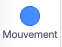
\includegraphics[width=1.5cm]{./images/scratch/mouvement.png} (colonne de gauche).
\item Tirer le bloc 
\includegraphics[width=2.5cm]{./images/scratch/BlocAllerA} vers la zone de programmation et l'accrocher sous le bloc 
\includegraphics[width=2.5cm]{./images/scratch/BlocDrapeauVert}.
\item Tirer ensuite le bloc 
\includegraphics[width=4.5cm]{./images/scratch/BlocGlisser} vers la zone de programmation et l'accrocher sous le bloc 
\includegraphics[width=2.5cm]{./images/scratch/BlocAllerA}.
\item Régler les options du bloc en cliquant dans les zones de saisie et en écrivant la valeur de durée et les coordonnées $x$ et $y$ indiquées dans le programme ci-dessus.
\item Ajouter les trois autres blocs 
\includegraphics[width=4.5cm]{./images/scratch/BlocGlisser} et régler leurs options comme indiqué plus haut.
\item Choisir les blocs de sons en cliquant sur 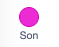
\includegraphics[width=1.5cm]{./images/scratch/son.png} (colonne de gauche).
\item Tirer le bloc 
\includegraphics[width=2.5cm]{./images/scratch/meow.png} vers la zone de programmation, l'accrocher aux blocs précédents et régler ses options comme indiqué plus haut.
\end{enumerate}

\vspace{12pt}

Après avoir terminé et vérifié le code, lancer le programme en appuyant sur le drapeau vert 
\includegraphics[width=.7cm]{./images/scratch/DrapeauVert} en haut à droite. Aviez-vous deviné correctement ce qu'il allait se passer ?

Pour arrêter l'exécution du programme avant sa fin, appuyer sur le panneau stop 
\includegraphics[width=.7cm]{./images/scratch/Stop} en haut.

Pour que le programme s'exécute en plein écran, cliquer sur 
\includegraphics[width=1cm]{./images/scratch/pleinEcran.png}\index{Scratch! Passer en mode plein écran}\index{Passer en mode plein écran (Scratch)}

Pour quitter le mode plein écran, cliquer sur 
\includegraphics[width=1cm]{./images/scratch/quitterPleinEcran.png}\index{Scratch! Quitter le mode plein écran}\index{Quitter le mode plein écran (Scratch)}








\subsubsection{Ajouter un code associé à la scène}\index{Scratch!Script associé à la scène}\index{Script associé à la scène (Scratch)}

Nous allons maintenant ajouter un deuxième code à notre programme : ce code va permettre de modifier la scène lorsque le drapeau vert est pressé. 

Pour cela, la première étape est de cliquer sur l'icône scène 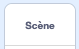
\includegraphics[width=1.5cm]{./images/scratch/scene0.png} en bas à droite.

\uneimageici{./images/scratch/premierProgramme2.png}{.7\textwidth}

Une fois la scène sélectionnée (elle est alors entourée en couleur), créer le code suivant :

\uneimageici{./images/scratch/ScratchProgramme1Script2}{.4\textwidth}

Une fois le code écrit et vérifié, lancer le programme en appuyant sur le drapeau vert 
\includegraphics[width=.7cm]{./images/scratch/DrapeauVert} en haut. 








%
%
%  S  É  A  N  C  E     II
%
%









\subsection{Aide pour la séance 2...}\label{correction_scratch2}


Construire le code : puisqu'il est associé à l'objet sprite, vérifier qu'il est bien sélectionné avant de le construire (voir si nécessaire le paragraphe \vref{ScriptLutin} pour sélectionner le lutin avant de construire le programme). Pour construire le bloc 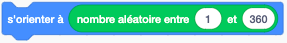
\includegraphics[width=6cm]{./images/scratch/scratchActivite2_0.png}, il faut procéder en deux temps :

\begin{enumerate}
\item Positionner les deux blocs d'instructions \texttt{s'orienter à...} et \texttt{nombre aléatoire entre...} dans la zone de programme ;

\uneimageici{./images/scratch/scratchActivite2_1.png}{.35\textwidth}

\item Tirer le bloc \texttt{nombre aléatoire entre...} dans la zone de saisi du bloc \texttt{s'orienter à...}

\uneimageici{./images/scratch/scratchActivite2_2.png}{.45\textwidth}

Il suffit ensuite de régler les valeurs et d'accrocher le bloc obtenu sous le bloc \texttt{abaisser le stylo}.
\end{enumerate}



Une fois que vous avez terminé et vérifié le code, lancer le programme en appuyant sur le drapeau vert 
\includegraphics[width=.7cm]{./images/scratch/DrapeauVert} en haut. Aviez-vous deviné correctement ce qu'il allait se passer ?




\subsubsection{Ajouter l'effacement de l'écran}

À côté du code précédent, construire le code ci-dessous qui permet d'effacer l'écran lorsque la touche \texttt{Espace} est pressée.

\uneimageici{./images/scratch/effacerTout.png}{.3\textwidth}

A noter que pour accéder aux fonctionnalités du stylo, on peut utiliser l'icône \texttt{Ajouter une extension} en bas à gauche 
\includegraphics[width=1cm]{./images/scratch/ajouterStylo.png}






\subsubsection{Un carré où on veut !}

En utilisant les instructions ci-dessous, modifier le code pour que le carré soit dessiné à l'endroit où se trouve le pointeur de la souris.

\uneimageici{./images/scratch/carreOuOnVeut.png}{.3\textwidth}


\subsubsection{Dessiner une enveloppe}

Créer un nouveau code, toujours pour l'objet sprite, qui permette de dessiner une enveloppe identique à celle ci-dessous. Le but est de réaliser cette enveloppe sans jamais lever le crayon ni repasser deux fois sur le même trait.

\uneimageici{./images/scratch/enveloppe}{.25\textwidth}




\subsubsection{Modifier la taille et la couleur du stylo}

En utilisant les instructions suivantes, modifier la couleur des traits et la taille du crayon.

\uneimageici{./images/scratch/modifierTailleStylo.png}{.4\textwidth}










%
%
%  S  É  A  N  C  E     III
%
%









\subsection{Aide pour la séance 3...}\label{correction_scratch3}



\subsubsection{Ajouter un nouvel objet}\index{Scratch!Ajouter et éditer un objet}\index{Ajouter et éditer un objet (Scratch)}

\begin{enumerate}
\item Cliquer sur l'icône \texttt{Choisir un sprite} 
\includegraphics[width=1cm]{./images/scratch/sprite.png}, puis sélectionner le costume que vous souhaitez.
\item Par exemple dans l'onglet \texttt{Animaux}, choisir \texttt{Parrot-a} 
\includegraphics[width=1cm]{./images/scratch/parrot.png}.
\uneimageici{./images/scratch/costumeParrot.png}{.8\textwidth}
\item Supprimer alors le sprite chat \texttt{Sprite0} en cliquant sur le bouton ''poubelle'' liée à ce sprite 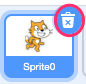
\includegraphics[width=1.5cm]{./images/scratch/poubelleChat.png}
%\uneimageici{./images/scratch/ScratchSupprimerLutin}{.5\textwidth}
\item Modifier la taille de votre sprite en remplaçant 100 par 50 dans la rubrique \texttt{Taille}. Vous pouvez également changer le nom de votre objet en l'appelant par exemple \texttt{Sprite1} dans la rubrique \texttt{Sprite}, et en appuyant sur la touche \texttt{Entrée} de votre clavier.
%Appuyer sur le bouton \texttt{Édition} à côté de l'avion, puis réduire la taille de l'avion en appuyant 8 fois sur le bouton 
\includegraphics[width=1cm]{./images/scratch/Reduire} :
\uneimageici{./images/scratch/reduireTaille.png}{.5\textwidth}
\end{enumerate}
On a maintenant un plus petit perroquet (objet remplaçant le chat), sur un fond blanc (objet scène).

Vérifier que l'objet \texttt{Sprite1} est bien sélectionné et cliquer sur l'onglet \texttt{Code} :

\uneimageici{./images/scratch/selectionCode.png}{.5\textwidth}






\subsubsection{Gérer les mouvements du perroquet dans la scène}  

On va maintenant ajouter un code pour notre perroquet. Puisque durant la partie, le perroquet doit toujours avancer, nous allons utiliser une \textbf{boucle infinie}.\index{Scratch!Boucle infinie}\index{Boucle infinie (Scratch)}

\vspace{12pt}

\cadre{La \textbf{boucle} est une structure importante en programmation : elle permet de répéter un bloc d'instructions plusieurs fois, tant qu'une condition est vérifiée ou même indéfiniment. Dans notre programme, nous utilisons une boucle infinie.\uneimageici{./images/scratch/ScratchBoucle}{.6\textwidth}}  

\vspace{12pt}



\begin{enumerate}
\item Construire le code suivant associé à l'objet perroquet (il faut donc que l'objet perroquet soit sélectionné) :
\uneimageici{./images/scratch/ScratchActivite31}{.3\textwidth}
\item Ajouter les deux codes suivants, également associés à l'objet perroquet :
\uneimageici{./images/scratch/ScratchActivite32}{.7\textwidth}
\item Pour tester votre programme, démarrer en appuyant sur le drapeau vert 
\includegraphics[width=.7cm]{./images/scratch/DrapeauVert} en haut. Appuyer sur le panneau stop 
\includegraphics[width=.7cm]{./images/scratch/Stop} en haut pour mettre fin au programme.
\end{enumerate}

Pour que le programme s'exécute en plein écran, cliquer sur 
\includegraphics[width=1cm]{./images/scratch/pleinEcran.png}\index{Scratch! Passer en mode plein écran}\index{Passer en mode plein écran (Scratch)}

Pour quitter le mode plein écran, cliquer sur 
\includegraphics[width=1cm]{./images/scratch/quitterPleinEcran.png}\index{Scratch! Quitter le mode plein écran}\index{Quitter le mode plein écran (Scratch)}

%Pour que le programme s'exécute en plein écran, cliquer sur 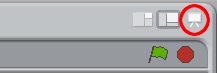
\includegraphics[width=3cm]{./images/scratch/ScratchPleinEcran}

%Pour quitter le mode plein écran, cliquer sur 
\includegraphics[width=1.5cm]{./images/scratch/ScratchQuitterPleinEcran}


\subsubsection{Un nouvel objet : l'obstacle}\index{Scratch!Créer un objet}\index{Créer un objet (Scratch)}       

On va maintenant ajouter un obstacle que le perroquet devra éviter.

\begin{enumerate}
\item Ajouter un nouvel objet en appuyant sur  
\includegraphics[width=1cm]{./images/scratch/sprite.png}. Choisir maintenant par exemple comme obstacle un \texttt{Paddle}
\uneimageici{./images/scratch/paddle.png}{.3\textwidth}
%\item Créer un petit rectangle de la couleur de votre choix.
%\uneimageici{./images/scratch/ScratchCreerRectangle}{.6\textwidth}
%Terminer en appuyant sur le bouton \texttt{OK}
\item Nous avons maintenant un nouvel objet nommé \texttt{Paddle}, présent dans la rubrique des sprites à gauche de l'écran.
%\uneimageici{./images/scratch/ScratchActivite34}{.4\textwidth}
\item Sélectionner à nouveau l'objet \texttt{Sprite1} car c'est à lui que nous allons associer un nouveau code.
\end{enumerate}


\subsubsection{Gérer la collision entre le perroquet et l'obstacle}\index{Scratch!Collision entre objets}\index{Collision entre objets (Scratch)} 

On va maintenant traiter le cas où le perroquet entre en collision avec l'obstacle. La partie sera alors perdue. Nous allons utiliser ici une \textbf{structure conditionnelle} : un bloc d'instructions sera exécuté \emph{si} la condition \emph{Sprite1 percute Paddle} est vérifiée.\index{Scratch!Structure conditionnelle \emph{si}}\index{Structure conditionnelle \emph{si} (Scratch)} 

\vspace{12pt}

\cadre{La \textbf{structure conditionnelle <<\,si\,>>} est une structure importante en programmation : elle permet d'exécuter un bloc d'instructions \textbf{si} une condition est vérifiée.\uneimageici{./images/scratch/ScratchSi}{.55\textwidth}}  

\vspace{12pt}





\begin{enumerate}
\item Modifier le code pour qu'il corresponde à celui ci-dessous. Le bloc 
\includegraphics[width=2cm]{./images/scratch/BlocCapteur} se trouve dans les blocs \texttt{Capteur} (colonne de gauche).
\uneimageici{./images/scratch/codeTouche.png}{.35\textwidth}
\item On ne veut pas le son par défaut \texttt{miaou} mais plutôt un son qui annonce que la partie est perdue. Pour cela, il faut enregistrer un nouveau son. Cliquer sur la flèche à droite du nom du son...
\uneimageici{./images/scratch/ScratchActiviteSonChanger}{.2\textwidth}

...puis choisir \texttt{enregistrer...}

\uneimageici{./images/scratch/enregistrerSon.png}{.3\textwidth}
\item Démarrer l'enregistrement à l'aide du bouton 
\includegraphics[width=1cm]{./images/scratch/boutonEnregistrer.png}, dire \emph{<<\,Perdu !\,>>}, puis l'arrêter à l'aide du bouton 
\includegraphics[width=2cm]{./images/scratch/boutonArret.png}. Faire plusieurs essais jusqu'à être satisfait du son enregistré.
\uneimageici{./images/scratch/essaiEnregistrement.png}{.6\textwidth}
\item Un nouveau son nommé \texttt{recording1} est maintenant disponible. %On peut alors supprimer le son \texttt{miaou} en cliquant sur le bouton 
\includegraphics[width=.7cm]{./images/scratch/Supprimer} :
\uneimageici{./images/scratch/recording1.png}{.5\textwidth}
\item On ajoute encore un quatrième et dernier code associé à \texttt{Sprite1}. Ce script permet de repositionner le perroquet lorsque la touche \texttt{espace} est pressée :
\uneimageici{./images/scratch/ScratchActivite39}{.3\textwidth}
\end{enumerate}













